\documentclass[tikz, margin=3.14mm]{standalone}

\usepackage{tikz}
\usetikzlibrary{decorations, calc, arrows, arrows.meta, positioning}

\begin{document}
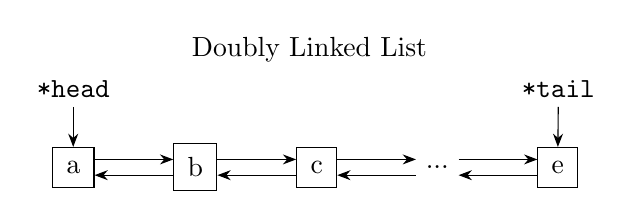
\begin{tikzpicture}[
    >=Stealth,
    list/.style={rectangle, draw, inner sep=5pt, text=black}
]

    % Nodes ------------------------------------------------------

    \node (title) at (3,1.5) {Doubly Linked List};
    \node[list] (n1) {a};
    \node (start) at (0, 1) {\texttt{*head}};
    \node[list, right=of n1] (n2) {b};
    \node[list, right=of n2] (n3) {c};
    \node[right=of n3] (n4) {...};
    \node[list, right=of n4] (n5) {e};
    \node (end) at (6.16, 1) {\texttt{*tail}};

    % Arrows ---------------------------------------------------

    % Down arrows
    \draw [->] ($(n1.east)+(0,.1)$) -- ($(n2.west)+(0,.1)$);
    \draw [->] ($(n2.east)+(0,.1)$) -- ($(n3.west)+(0,.1)$);
    \draw [->] ($(n3.east)+(0,.1)$) -- ($(n4.west)+(0,.1)$);
    \draw [->] ($(n4.east)+(0,.1)$) -- ($(n5.west)+(0,.1)$);

    % Down arrows
    \draw [->] ($(n2.west)-(0,.1)$) -- ($(n1.east)-(0,.1)$);
    \draw [->] ($(n3.west)-(0,.1)$) -- ($(n2.east)-(0,.1)$);
    \draw [->] ($(n4.west)-(0,.1)$) -- ($(n3.east)-(0,.1)$);
    \draw [->] ($(n5.west)-(0,.1)$) -- ($(n4.east)-(0,.1)$);

    % Pointer labels
    \draw [->] (end.south) -- (n5.north);
    \draw [->] (start.south) -- (n1.north);

\end{tikzpicture}
\end{document}